\begin{savequote}[6cm]
<< Doing things didn't work, not doing things didn't work, and I couldn't predict the future either, so I only had one other choice. \textbf{Monitor everything}. >>
\qauthor{Twilight Sparkle}
\end{savequote}
\chapter{Contexte et objectifs de la thèse}
\chaptertoc

Ce premier chapitre replace brièvement le contexte de cette thèse en section~\ref{sec:intro:contexte}. Puis, nous détaillons les problématiques de recherche en section~\ref{sec:intro:problematique}. Ensuite, nous présentons notre cadre applicatif que nous utilisons en section~\ref{sec:introduction:digitalhome}. Nous présentons la démarche adoptée et les principales contribution de ce travail en section~\ref{sec:intro:demarche}, et enfin, nous détaillons le plan de ce manuscrit en section~\ref{sec:intro:plan}.

\section{De l'importance de la supervision}\label{sec:intro:contexte}
%    Systèmes de plus en plus complexes

L'informatique a évolué de façon drastique au cours de ces dernières années. Grâce à l'amélioration des technologies de la micro-électronique, du réseau, et évidemment des techniques logicielles, il est désormais possible de concevoir des systèmes tels que :
\begin{itemize}
 \item Un réseau de capteurs. De nombreux micro-dispositifs autonomes, ou à durée de vie longue, capables de transmettre des informations sur une quantité physique sans fils. Ensembles, ils sont capables de créer un système de surveillance dans le cadre par exemple de l'agriculture de précision.
 \item Un environnement domestique intelligent. Grâce aux technologies sans-fil ou courant-porteur, des dispositifs sont capables de communiquer pour fournir des services de haut-niveaux. De tels services peuvent être  multimédia tels que le partage de flux vidéos ou la visiophonie. Mais aussi, ils peuvent être plus orienté sur l'amélioration du confort de vie de l'usager comme la gestion automatique des lumières ou encore l'assistance aux personnes handicapées.
 \item Un centre de traitement de données. Que ce soit pour virtualiser des services à très large échelle ou pour établir une ferme de calcul scientifique, la mise en relation de centaines d'équipements informatiques permet d'effectuer des traitements complexes.
\end{itemize}

%    Interactions nombreuses et volatiles
Ainsi, l'ordinateur personnel n'est plus qu'une partie des possibles interactions qu'un utilisateur quelconque peut faire avec l'informatique. Ces systèmes partagent la caractéristique principale suivante~: ces sont des dispositifs qui interagissent via un réseau pour fournir un service de haut niveau. Ces interactions sont nombreuses et potentiellement volatiles. Afin de mieux comprendre ces systèmes, il est nécessaire de les observer.

%    Établissement d'un diagnostic
La supervision d'un système est le processus en charge de collecter, traiter, et éventuellement stoquer les données relatives à un système pour en vérifier son bon fonctionnement. Cette surveillance peut s'effectuer en temps réel afin d'être pro-actif sur la réaction aux événements importants, ou par analyse a posteriori sur l'ensemble des données qui ont été collectées. Ainsi, lorsqu'un problème surgit sur un système, critique ou non, ce procédé est au cœur de la résolution de problèmes. En effet, si le traitement est en temps réel pourra détecter l'anomalie et pourra transmettre l'information à qui est capable d'y remédier (l'utilisateur ou système tiers). Sinon, il sera possible de retracer l'origine du problème par le parcours des données collectées afin d'établir un diagnostic.

%    Aide à l'administration
Enfin, la supervision est un outil central lors de l'administration du système. En effet, comme la surveillance passe aussi par la gestion de la configuration de chacun des dispositifs et services, il devient une base précieuse d'informations pour l'aide à la gestion du système car cela permet à l'administrateur d'avoir une vue détaillée du fonctionnement de son système.

Toutefois, le processus de surveillance doit être capable de répondre à la diversité et la grandissante complexité des systèmes informatiques. L'enjeu principal étant la capacité du système de supervision à s'adapter à l'hétérogénéité des systèmes, des dispositifs et des données. La section suivante présente plus en détail la problématique de cette thèse.
\section{L'hétérogénéité au cœur du problème}\label{sec:intro:problematique}
La supervision est un processus qui est nécessaire et applicable à une grande quantité de domaine. Cela ouvre la porte à la problématique majeure de cette thèse : la diversité des applications. Cela a pour conséquence une hétérogénéité à plusieurs niveau. Cette section développe les trois axes majeurs de diversité en terme de : systèmes (section~\ref{sec:intro:problematique:devices}), besoins d'observation (section~\ref{sec:intro:problematique:observation}) et enfin en terme de données (section~\ref{sec:intro:problematique:data}).

\subsection{Une grande variété de systèmes et dispositifs}\label{sec:intro:problematique:devices}
Plus l'informatique évolue, plus le nombre de dispositifs créés varie. Grâce à l'émergence de l'informatique ubiquitaire, les dispositifs se font de plus en plus nombreux et de natures complètement différentes. Ces caractéristiques rendent leur observation plus délicate car la surveillance des données d'un capteur est sensiblement différente à celle de l'utilisation d'un service d'hébergement web sur un serveur grande capacité. D'une part, les ressources utilisables pour extraire les données seront plus limités sur le capteur, augmentant ainsi le risque d'ingérence dans le fonctionnement du système. D'autre part, la nature des méthodes de collecte des données pourra être très variée, en terme de protocole d'accès, comme de mode d'interrogation (\textit{push} ou \textit{pull}).

D'un point de vue structurel, les dispositifs ne sont pas composés de la même manière. Alors qu'un capteur pourra être modélisé avec quelques variables d'états (niveau de batterie, valeur numérique du capteur, puissance signal radio, ...), un décodeur TV est quant à lui beaucoup plus complexe par essence. En effet, il est composé de modules matériels, d'un système logiciel, de divers applications et de modules de communications. Chacune de ces entités regorge de variables d'états potentiellement à surveiller, suivant l'application. Ainsi, l'hétérogénéité des dispositifs ouvre la voie à une grande diversité d'entités complexes à observer.

De plus, la mise en communication de ces divers dispositifs fait encore augmenter la complexité d'un système complet de manière exponentielle. Comme présenté précédemment, des capteurs sont capables de former un réseau qui peut lui même communiquer avec d'autres équipements domotiques ou avec un serveur d'application distant. Ainsi, la structure même du système est hétérogène car dans le cas présenté, la communication entre les équipements ne se fera pas directement suivant les cas. Ainsi, il est nécessaire de représenter les différentes connections possibles ou établies entre les dispositifs, qui elles-mêmes possèdent des caractéristiques. 

La description des différentes entités du système et leurs liens compose ainsi une structure complexe du système. Cette structure est malheureusement attaché par nature au système et variera d'une application à l'autre.

\subsection{Les perspectives d'observations}\label{sec:intro:problematique:observation}
La supervision ne se justifie que par l'utilisation qui en est faite et par son application. En effet, pour tout système, il existe plusieurs angles de vues possibles. Cet angle définira par la suite les données surveillées mais aussi la représentation du système.

Par exemple, lors de l'observation d'un système domotique. Un expert réseau s'intéressera aux liens entre les dispositifs, à la qualité de ces liens, et évidemment à l'évolution de la topologie. Alors qu'un expert multimédia s'intéressera lui au matériel de TV, aux logiciels d'encodage/décodage et aux intergiciels de partages de contenus. Les conséquences sont majeures car dans le premier cas, la représentation qui sera faite du système sera principalement un graphe annoté (la topologie, les propriétés des nœuds et liens). Alors que dans le deuxième cas, la représentation pourra être un modèle de classe extrait du domaine du multimédia.

Choisir un point de vue permet de restreindre la complexité inhérente au système observé. Toutefois, il est nécessaire que la supervision s'adapte aux perspectives dans lesquelles se placent les experts. Ainsi une grande flexibilité est nécessaire pour gérer cette diversité de besoins.

\subsection{Les données}\label{sec:intro:problematique:data}
La perspective d'observation fixe ainsi l'ensemble des données qu'il est nécessaire de gérer pour répondre aux besoins d'observations. Cependant, cet ensemble est d'une grande hétérogénéité suivant plusieurs axes :
\begin{itemize}
 \item \textbf{Syntaxe} : Il apparaît naturel qu'une grande diversité syntaxique soit présente sur l'ensemble de données. Un capteur renseignera son relevé avec une valeur numérique, tandis qu'une carte réseau donnera son adresse \textit{IP} (v4 ou v6), et un serveur d'application sera capable de fournir un rapport sous forme complexe (document \textit{XML} ou \textit{JSON}). À chacun de ces types, plusieurs opérations deviennent possibles. Une valeur numérique pourra, souvent, être agrégée via des fonctions statistiques, alors qu'un document \textit{XML} pourra être lui décomposé par nœud.
 \item \textbf{Sémantique} : Chaque donnée a une sémantique propre définie par son attachement à différents concepts. Par exemple, la donnée \textit{Statut} indiquant l'état d'un objet, n'aura de sens que si elle est liée à une entité du système comme : le statut du service décodage TV. Des liens sémantiques peuvent être tissés entre les données afin de définir des contraintes ou des règles de fonctionnement. Ainsi, il peut être défini que le statut de l'équipement de décodage TV est intrinsèquement associé au statut du service décodage TV. 
 \item \textbf{Pertinence} : Devant la masse de données pouvant être présente dans le système observé, il est nécessaire d'extraire les quelques éléments pertinents pour répondre aux besoins de l'expert. De ce fait, chaque donnée ne partage pas la même importance aux yeux de l'utilisateur. Dans le cadre de la surveillance de fonctionnement, la notification d'un dépassement de seuil d'une variable d'état critique aura certainement plus de pertinence que le numéro de série d'un équipement. Il est important de noter que ceci est très dépendant de la perspective d'observation car dans le cas de l'aide à l'administration d'un parc de dispositifs, le numéro de série aura beaucoup de valeur.
 \item \textbf{Dynamique} : Une donnée n'est pas toujours statique dans le temps. En effet, son évolution implique des conséquences directe sur sa sémantique et son importance, modifiant ainsi son traitement. Quatre dynamiques principales sont identifiables.
    \begin{itemize} 
        \item \textit{Événementielle} : la donnée survient uniquement de manière non-prédictible. Ces événements ont de l'importance car ils traduisent un comportement particulier du système pouvant être une alerte ou un changement d'état brusque, ce qui est très pertinent pour de l'observation.
        \item \textit{Régulière} : la mise à jour se fera suivant un schéma connu et prédictible, par exemple, un capteur envoie sa mesure toutes les cinq secondes. L'importance de cette donnée sera visible principalement en considérant l'ensemble de son historique et non la donnée figée à un instant précis.
        \item \textit{Stable} : la donnée ne changera que très rarement, c'est le cas des informations de configurations comme la version d'un logiciel. Lors de l'établissement d'un diagnostic, l'état courant de ce type de variable est pertinent pour analyser. Il est important de noter que pour certaines données critique, l'action de mise à jour peut constituer un événement qui sera nécessaire de traiter.
        \item \textit{Statique} : la donnée ne changera jamais sous toute condition comme le numéro de série d'un équipement, ou les informations constructeurs. Ce type d'information est nécessaire si l'application de surveillance justifie l'utilisation d'une description du système.
    \end{itemize}
\end{itemize}

En conclusion, le système de supervision doit être capable de s'adapter à tout type de système informatique ainsi qu'aux angles de vues des experts métiers. Une fois ce contexte d'utilisation correctement défini, il est nécessaire de gérer la grande diversité de données présente, que ce soit en terme de type, de sémantique ou d'évolution temporelle. Ces différents aspects de la données impliqueront des conséquences directes sur sa pertinence.

\section{Domaine d'application : le réseau local domestique}\label{sec:introduction:digitalhome}
Cette thèse a été développée dans un milieu industriel chez \textit{Orange Labs}. Les propositions de cette thèse sont génériques, mais grâce à ce contexte de travail, nous avons pu appliquer notre approche dans un domaine applicatif qui pose actuellement de nombreux problèmes : le réseau domestique (ou \textit{Digital Home}).

\begin{figure}[ht]
\centering
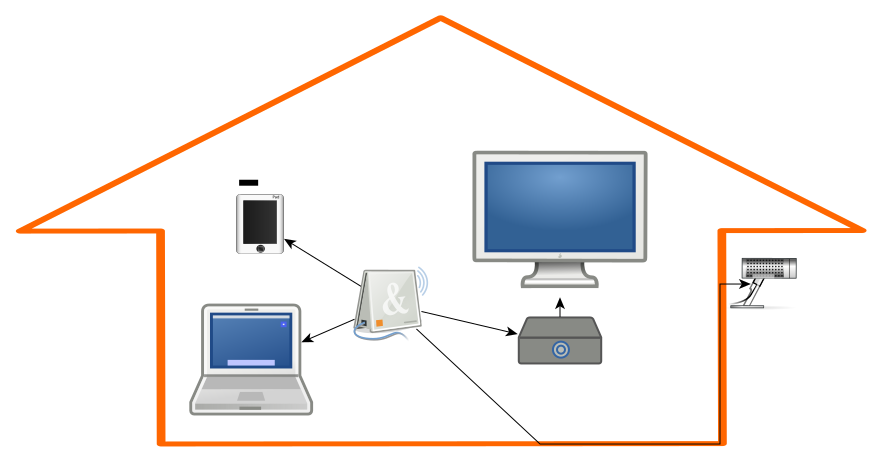
\includegraphics[width=0.7\textwidth]{intro-digitalhome}
\caption{Exemple de réseau domestique}
\end{figure}

Le réseau domestique est formé par l'ensemble des appareils se trouvent dans une maison. Ce réseau est déjà capable de fournir des services tels que le partage de contenus entre un disque dur en réseau (ou \textit{NAS}) sur la télévision ou sur les ordinateurs. L'étape suivante du développement de cette approche est l'introduction de capteurs et d'actuateurs (domotique).

Les opérateurs télécoms qui fournissent des équipements et des services sont bien souvent en difficultés pour dépanner les utilisateurs. Une des raisons de ce problème est notamment le manque d'informations sur le système. Le service après-vente ne possède pas de moyen de connaître la topologie du réseau (utilisation de \textit{wifi} ou courant porteur), la configuration de certains équipements et encore moins l'état de fonctionnement des équipements, des liens réseau ou des services.

Ce cadre applicatif a fourni les cas d'études et d'expérimentation à cette thèse. Ils réunissent les caractéristiques que nous avons introduites en~\ref{sec:intro:problematique}.
\begin{itemize}
	\item Le réseau domestique est composé de dispositifs hétérogènes.
	\item Chaque équipement fournit ses propres données sous des schémas que nous ne maîtrisons pas.
	\item Les paramètres de configuration et d'autres données accessibles via des services spécifiques sont des données persistantes. Il est possible de récupérer des données de métriques pour mesurer la santé du réseau.
	\item Des requêtes hybrides sont nécessaire pour former des alarmes basées sur des données persistantes (catalogue, agrégats historiques).
	\item Plusieurs types d'utilisateurs avec des métiers différents observent ce réseau.
\end{itemize}

Les travaux développés dans cette thèse contribuent à un système d'observation applicable sur tout système. Nous validerons notre approche par son application sur la compréhension du réseau local domestique. Ceci pourra être utilisé pour aider les diagnostics faits au service après-vente.

\section{Approche et contributions de cette thèse}\label{sec:intro:demarche}
Nous proposons une approche orientée donnée pour l'observation de systèmes. En particulier, nous nous sommes orientés sur le domaine de la gestion des flux de données. Ceci nous permet de créer un langage algébrique unique d'interrogation pour toutes les catégories de données (persistantes et temps réel). Grâce à ce langage, nous développons un intergiciel capable de gérer les données issues de l'observation. Cette section présente brièvement nos contributions.

\subsection{Un langage unique d'interrogation}
La gestion de flux de données est un domaine permettant de gérer de manière déclarative les données temps-réel. Cette approche permet une grande souplesse, car il est possible de déployer des requêtes complexes via un langage déclaratif sur les données. Toutefois, les langages manquent encore de fondations théoriques pour correctement maîtriser ses données.

Nous avons spécifié une algèbre permettant d'interroger de manière unifiée les données sous forme de flux ou relations de bases de données. Elle a pour propriété d'être capable de manipuler les deux modes d'interrogation sur des données persistantes ou temps réel. De plus, ces définitions sont déterministes. Ainsi, lors de l'expression d'une requête par cette algèbre, il n'existe qu'une interprétation du résultat, ce qui permet une gestion plus claire de ses données.

\subsection{Un intergiciel extensible d'évaluation de requête}
Il existe plusieurs intergiciels capables d'évaluer des requêtes continues sur les systèmes de gestions de flux de données. Toutefois, leur implémentation peut influencer les sémantiques d'évaluations de requête. Des approches existent pour intégrer des évaluateurs d'un point de vue architectural. Toutefois, il existe peu d'approches pour spécifier formellement le comportement d'un opérateur d'un évaluateur.

Nous proposons un intergiciel capable d'évaluer des requêtes exprimées dans le langage algébrique que nous avons développé. Cette algèbre nous sert aussi pour la spécification des composants de l'intergiciel. En effet, chaque module implémentant un opérateur doit spécifier sa sémantique selon une ou plusieurs règles se basant sur des opérateurs algébriques. Ce principe couplé avec les notions architecturales de composants orientés services nous permettent d'avoir une grande flexibilité pour permettre aux utilisateurs de personnaliser au mieux cette solution.

De plus, notre approche à base de règle nous permet de développer une approche générale d'optimisation des requêtes. Tout comme en SGBD, nous appliquons une optimisation logique, puis physique de notre requête. Ces optimisations sont possibles grâce aux résultats d'équivalence de requête démontrable avec l'algèbre.

\subsection{Une intégration des supports persistants}
Enfin, nous avons vu que notre langage est capable d'interroger de manière unifiée les données temps réel et persistantes. Dans la littérature, plusieurs rapprochements existent entre les deux mondes de manière ad hoc ou implicite.

Grâce à notre langage, nous proposons une infrastructure capable d'intégrer un SGBD à notre intergiciel de gestion de flux. Ainsi, l'utilisateur doit spécifier le schéma du système observé, ainsi que des requêtes permettant l'intégration des données flux dans la base. À l'issue de ce travail de spécifications, l'utilisateur devient capable d'interroger les données persistantes et temps réel via l'algèbre. Il est alors garanti de la mise en œuvre de sa requête de façon efficace. Cette infrastructure est proposée comme extension de notre intergiciel.

\section{Plan de thèse}\label{sec:intro:plan}
\TODO{}
